%!TEX program = xelatex
\documentclass[11pt,a4paper]{article}
\usepackage[utf8]{inputenc}
\usepackage[T1]{fontenc}
\usepackage{ctex}
\usepackage{authblk}
\usepackage{tikz}
\usepackage{pgfplots}
\usepackage{verbatim}
\usepackage{amsfonts}
\usepackage{amsmath}
\usepackage{amsthm}
\usepackage{indentfirst}
\usepackage{amssymb}
\usepackage{enumerate}
\setlength{\parindent}{0pt}
\usetikzlibrary{shapes,snakes}
\newcommand{\argmax}{\operatornamewithlimits{argmax}}
\newcommand{\argmin}{\operatornamewithlimits{argmin}}

\DeclareMathOperator{\col}{col}
\usepackage{booktabs}
\newtheorem{theorem}{Theorem}
\newtheorem{proposition}{Proposition}
\newtheorem{lemma}{Lemma}
\newtheorem{example}{Example}
\newtheorem{corollary}{Corollary}
\newtheorem{definition}{Definition}
\newtheorem{note}{Note}
\newtheorem{claim}{Claim}
\usepackage{graphicx}
\usepackage{geometry}
\usepackage{hyperref}
\newcommand{\code}{	exttt}
\geometry{a4paper,scale=0.8}
\title{Optimization}
\author[*]{Wenxiao Yang}
\affil[*]{Department of Mathematics, University of Illinois at Urbana-Champaign}
\date{2022}





\begin{document}
\maketitle
\tableofcontents
\newpage

\section{Unconstrained Optimization}
\subsection{Conditions for Optimality}
Function: $f:\mathbb{R}^n \rightarrow	\mathbb{R}^n$, $x\in \&,\ \&\subseteq \mathbb{R}^n$.

Terminology: $x^*$ will always be the optimal input at some function.

\subsection{Global minimizer, Local minimizer}
\begin{definition}
    \quad\\
    Say $x^*$ is a \underline{global minimizer(minimum)} of $f$ if $f(x^*)\leq f(x), \forall x\in \&$.

    Say $x^*$ is a \underline{unique global minimizer(minimum)} of $f$ if $f(x^*)< f(x), \forall x\neq x^*$.

    Say $x^*$ is a \underline{local minimizer(minimum)} of $f$ if $\exists r>0$ so that $f(x^*)\leq f(x)$ when $\|x-x^*\|<r$.
\end{definition}

A minimizer is \underline{strict} if $f(x^*)< f(x)$ for all relevant $x$.

\subsection{Optimization in $\mathbb{R}$}
\subsubsection{Theorem: local minimizer $\Rightarrow f'(x^*)=0$}

\begin{theorem}
If $f(x)$ is differentiable function and $x^*$ is a local minimizer, then $f'(x^*)=0$.
\end{theorem}

\begin{proof}
\quad\\
Def of $f'(x)=\lim_{h \rightarrow 0} \frac{f(x+h)-f(x)}{h}$\\
Def of local minimizer: $f(x^*)-f(x)\geq 0, |x^*-x|<r$\\
when $0<h<r$, $\frac{f(x+h)-f(x)}{h}\geq 0$; when $-r<h<0$, $\frac{f(x+h)-f(x)}{h}\leq 0$. Then $f'(x)=0$.
\end{proof}

\subsubsection{Theorem: $f'(x^*)=0, f''(x^*)\geq 0 \Rightarrow$ local minimizer}
\begin{theorem}
    If $f:\mathbb{R} \rightarrow \mathbb{R}$ is a function with a continuous second derivative and $x^*$ is a critical point of $f$ (i.e. $f'(x)=0$), then:\\
    (1): If $f''(x)\geq 0,\ \forall x\in\mathbb{R}$, then $x^*$ is a global minimizer on $\mathbb{R}$.\\
    (2): If $f''(x)\geq 0,\ \forall x\in[a,b]$, then $x^*$ is a global minimizer on $[a,b]$.\\
    (3): If we only know $f''(x^*)\geq 0$, $x^*$ is a local minimizer.
\end{theorem}
\begin{proof}
\quad\\
(1)$f(x)=f(x^*)+f'(x^*)(x-x^*)+\frac{1}{2}f''(\xi)(x-x^*)^2=f(x^*)+0+\textit{something non negative}\geq f(x^*)\  \forall x$\\
(2) Similar to (1)\\
(3)$f''(x^*)\geq 0,\ f''$ continuous $\Rightarrow \exists r$ s.t. $f''(x)\geq 0$ $\forall x\in[x^*-\frac{r}{2},x^*+\frac{r}{2}]$, then $x$ is a local minimizer.
\end{proof}


\subsection{Optimization in $\mathbb{R}^n$}
\subsubsection{Necessary Conditions for Optimality: Local Extremum $\Rightarrow \nabla f(x^*)=0$}
A base point $x$, we consider an arbitrary direction $u$. $\{x+tu| t\in \mathbb{R}\}$

For $\alpha>0$ sufficiently small:
\begin{enumerate}
    \item $f(x^*)\leq f(x^*+\alpha u)$
    \item $g(\alpha)=f(x^*+tu)-f(x^*)\geq 0$
    \item $g(\beta)$ is continuously differentiable for $\beta\in[0,\alpha]$
\end{enumerate}

By chain rule, $$g'(\beta)=\sum_{i=1}^n \frac{\partial f}{\partial x_i}(x^*+\beta u)u_i$$

By Mean Value Theorem, $$g(\alpha)=g(0)+g'(\beta)\alpha\text{ for some }\beta\in[0,\alpha]$$
Thus $$g(\alpha)=\alpha\sum_{i=1}^n \frac{\partial f}{\partial x_i}(x^*+\beta u)u_i\geq 0$$
$$\Rightarrow \sum_{i=1}^n \frac{\partial f}{\partial x_i}(x^*+\beta u)u_i\geq 0$$
Letting $\alpha \rightarrow	0$ and hence $\beta \rightarrow	0$, we get $$\sum_{i=1}^n \frac{\partial f}{\partial x_i}(x^*)u_i\geq 0\text{ for all }u\in \mathbb{R}^n$$
By choosing $u=[1,0,...,0]^T$, $u=[-1,0,...,0]^T$, we get $$\frac{\partial f(x^*)}{\partial x_1}\geq 0,\ \frac{\partial f(x^*)}{\partial x_1}\leq 0 \Rightarrow	\frac{\partial f(x^*)}{\partial x_1}= 0$$
Similarly, we can get $$\nabla f(x^*)=[\frac{\partial f(x^*)}{\partial x_1},\frac{\partial f(x^*)}{\partial x_2},...,\frac{\partial f(x^*)}{\partial x_n}]^T=0$$

\begin{theorem}
If $f$ is continuously differentiable and $x^*$ is a local extremum. Then $\nabla f(x^*)=0$.
\end{theorem}

\subsubsection{Stationary Point, Saddle Point}
All points $x^*$ s.t. $\nabla f(x^*)=0$ are called \underline{stationary points}.

Thus, all extrema are stationary points.

But not all stationary points have to be extrema.

\underline{Saddle points} are the stationary points neither local minimum nor local maximum.

\begin{example}
$f(x)=x^3$, $x=0$ is a stationary point but not extrema. (saddle point)
\end{example}

\subsubsection{Second Order Necessary Condition}
\begin{definition}
The Hessian of $f$ at point $x$ is an $n\times n$ symmetric matrix denoted by $\nabla^2 f(x)$ with $[\nabla^2 f(x)]_{ij}=\frac{\partial^2 f(x)}{\partial x_i\partial x_j}$
\end{definition}
\begin{theorem}
Suppose $f$ is twice continuously differentiable and $x^*$ in local \underline{minimum}. Then $$\nabla f(x^*)=0\text{ and }\nabla^2 f(x^*)\succeq 0$$
\end{theorem}
\begin{proof}
\quad\\
$\nabla f(x^*)=0$ already proved before.

Let $\alpha$ be small enough so that $g(\alpha)=f(x^*+\alpha u)-f(x^*)\geq 0$.

By Taylor series expansion,
\begin{equation}
    \begin{aligned}
        g(\alpha)&=g(0)+\alpha g'(0)+\frac{\alpha^2}{2}g''(0)+O(\alpha^2)\\
        g'(\alpha)&=\sum_{i=1}^n \frac{\partial f}{\partial x_i}(x^*+\beta u)u_i=\nabla f(x^*+\alpha u)^T u\\
        g''(\alpha)&=\sum_{i=1}^n\sum_{j=1}^n \frac{\partial^2 f}{\partial x_i\partial x_j}(x^*+\beta u)u_iu_j=u^T\nabla^2 f(x^*+\alpha u) u
    \end{aligned}
    \nonumber
\end{equation}
\begin{equation}
    \begin{aligned}
        g'(0)=\nabla f(x^*)^T u=0;\ g''(0)=u^T\nabla^2 f(x^*) u\\
        g(\alpha)=\frac{\alpha^2}{2}u^T\nabla^2 f(x^*) u+O(\alpha^2)\geq 0\\
        \text{When }\alpha \rightarrow 0,\text{ we get } u^T\nabla^2 f(x^*) u\geq 0,\ \forall u\in \mathbb{R}^n\\
        \Rightarrow	\nabla^2 f(x^*)\succeq 0
    \end{aligned}
    \nonumber
\end{equation}
\end{proof}

\subsubsection{Sufficient Conditions for Optimality}
\begin{theorem}
Suppose $f$ is twice continuously differentiable in a neighborhood of $x^*$ and 
(1) $\nabla f(x^*)=0$; (2) $\nabla^2 f(x^*)\succ 0$ ($u^T\nabla^2 f(x^*) u>0$, $\forall u\in \mathbb{R}^n$).
Then $x^*$ is local minimum.
\end{theorem}
\begin{proof}
\quad\\
Consider $u\in \mathbb{R}^n$, $\alpha>0$ and let
\begin{equation}
    \begin{aligned}
        g(\alpha)&=f(x^*+\alpha u)-f(x^*)\\
        &=\frac{\alpha^2}{2}u^T\nabla^2 f(x^*) u+O(\alpha^2)\geq 0\\
        &=\frac{\alpha^2}{2}[u^T\nabla^2 f(x^*) u+2\frac{O(\alpha^2)}{\alpha^2}]\\
        &u^T\nabla^2 f(x^*) u>0;\ \frac{O(\alpha^2)}{\alpha^2}\rightarrow 0\\
        &\Rightarrow g(\alpha)>0\text{ for }\alpha\text{ sufficiently small for all }u\neq 0\\
        &\Rightarrow x^*\text{ is local minimum}.
    \end{aligned}
    \nonumber
\end{equation}

(specially if $\|u\|=1$, $u^T\nabla^2 f(x^*) u\geq \lambda_{\min}(\nabla^2 f(x^*))$, $\lambda_{\min}(\nabla^2 f(x^*))$ is the minimal eigenvalues of $\nabla^2 f(x^*)$.)
\end{proof}






\subsubsection{Using Optimality Conditions to Find Minimum}
\begin{enumerate}
    \item Find all points satisfying necessary condition $\nabla f(x)=0$ (all stationary points)
    \item Filter out points that don't satisfy $\nabla^2 f(x)\geq 0$
    \item Points with $\nabla^2 f(x)> 0$ are strict local minimum.
    \item Among all points with $\nabla^2 f(x)\geq 0$, declare a global minimum, one with the smallest value of $f$, assuming that global minimum exists.
\end{enumerate}
\begin{example}
$f(x)=2x^2-x^4$
\end{example}
\begin{equation}
    \begin{aligned}
        f'(x)&=4x-4x^3=0\\
        \Rightarrow& x=0,x=1,x=-1\text{ are stationary points}\\
        f''(x)&=4-12x^2=\left\{\begin{matrix}
            4&\text{if }x=0\\
            -8&\text{if }x=1,-1
        \end{matrix}\right.\\
        \Rightarrow	&x=0\text{ is the only local min, and it is strict}
    \end{aligned}
    \nonumber
\end{equation}
But $-f(x) \rightarrow \infty$ as $|x|\rightarrow \infty \Rightarrow$ no global min, but global max exists. $f(1),f(-1)$ are strict local max and both global max.

\subsubsection{Fix Conditions for Global Optimality}
\textbf{Claim 1}: Consider a differentiable function $f$. Suppose:

(C1) $f$ has at least one global minimizer;

(C2) The set of stationary points is $S$, and $f\left(x^{*}\right) \leq f(x), \forall x \in S$.

Then $x^{*}$ is a global minimizer of $f^{*}$.
\begin{proof}
\quad\\
Suppose $\hat{x}$ is a global minimizer of $f$, i.e.,
$$
f(\hat{x}) \leq f(x), \forall x .
$$
By the necessary optimality condition, we have $\nabla f(\hat{x})=0$, thus $\hat{x} \in S$. By (C2), we have
$$
f\left(x^{*}\right) \leq f(\hat{x}) .
$$
Combining the two inequalities, we have $f(\hat{x}) \leq f\left(x^{*}\right) \leq f(\hat{x})$, thus $f(\hat{x})=f\left(x^{*}\right)$. Plugging into the second inequality, we have $f\left(x^{*}\right) \leq f(x), \forall x$. Thus $x^{*}$ is a global minimizer of $f^{*} .$
\end{proof}



\subsection{Optimization in a Set}
$$\begin{array}{ll}\text { minimize } & f(x) \\ \text { subject to } & x \in X\end{array}$$
- Objective function $f: \mathbb{R}^{n} \rightarrow \mathbb{R}$ is a continuous function

- Optimization variable $x \in X$

- Local minimum of $f$ on $X: \exists \epsilon>0$ s.t. $f(x) \geq f(\hat{x})$, for all $x \in X$ such that $\|x-\hat{x}\| \leq \epsilon$;

i.e., $x^{*}$ is the best in the intersection of a small neighborhood and $X$

- Global minimum of $f$ on $X: f(x) \geq f\left(x^{*}\right)$ for all $x \in X$

"Strict global minimum", "strict local minimum" "local maximum", "global maximum" of $f$ on $X$ are defined accordingly

\subsubsection{Existence of Global-min}
\begin{theorem}[Bolzano-Weierstrass Theorem (compact domain)]
    Any continuous function $f$ has at least one global minimizer on any \textbf{compact set} $X$.

    That is, there exists an $x^{*} \in X$ such that $f(x) \geq f\left(x^{*}\right), \forall x \in X$.
\end{theorem}

\begin{corollary}[bounded level sets]
    Suppose $f: \mathbb{R}^{d} \rightarrow \mathbb{R}$ is a continuous function. If for a certain $c$, the level set
    $$
    \{x \mid f(x) \leq c\}
    $$
    is \textbf{non-empty} and \textbf{compact}, then the global minimizer of $f$ exists, i.e., there exists $x^{*} \in \mathbb{R}^{d}$ s.t.
    $$
    f\left(x^{*}\right)=\inf _{x \in \mathbb{R}^{d}} f(x)
    $$
\end{corollary}
\begin{example}
    $f(x) = x^2$.
    Level set $\{x|x^2 \leq 1\}$ is $\{x|−1\leq x\leq 1\}$: non-empty compact. Thus there exists a global minimum.
\end{example}
\begin{corollary}[coercive]
    Suppose $f: \mathbb{R}^{d} \rightarrow \mathbb{R}$ is a continuous function. If $f(x) \rightarrow \infty$ as $\|x\| \rightarrow \infty$, then the global minimizer of $f$ over $\mathbb{R}^{d}$ exists.
\end{corollary}
\begin{proof}
Let $\alpha\in \mathbb{R}^d$ be chosen so that the set $S = \{x |f(x) \leq \alpha\}$ is non-empty. By coercivity,
this set is compact.
\end{proof}
Coercive $\Rightarrow$ one non-empty bounded level set; but not the other way.

Claim (all level sets bounded $\Leftrightarrow$ coercive): Let $f$ be a continuous function, then $f$ is coercive iff $\{x | f(x) \leq \alpha\}$ is compact for any $\alpha$.

\subsection{Method of finding-global-min-among-stationary-points (FGMSP)}
Method of finding-global-min-among-stationary-points (FGMSP):

Step 0: Verify coercive or bounded level set:

- Case 1: success, go to Step $1 .$

- Case 2: otherwise, try to show non-existence of global-min. If success, exit and report "no global-min exists".

- Case 3: cannot verify coercive or bounded level set; cannot show non-existence of global-min. Exit and report "cannot decide".

Step 1: Find all stationary points (candidates) by solving $\nabla f(\mathbf{x})=0$;

Step 2 (optional): Find all candidates s.t. $\nabla^{2} f(\mathbf{x}) \succeq 0$.

Step 3: Among all candidates, find one candidate with the minimal value. Output this candidate, and report "find a global $\mathrm{min}$ ".






\section{Convexity}
\subsection{Definition}
\textbf{Convex set} $C: x, y \in C$ implies $\lambda x+(1-\lambda) y \in C$, for any $\lambda \in[0,1]$.

\textbf{Convex function} (0-th order): $f$ is convex in a convex set $C$ iff $f(\alpha x+(1-\alpha) y) \leq \alpha f(x)+(1-\alpha) f(y), \forall x, y \in C, \forall \alpha \in[0,1] .$

Property (1st order) If $f$ is differentiable, then $f$ is convex iff $f(z) \geq f(x)+(z-x)^{T} \nabla f(x), \ \forall x, z \in C .$ The inequality is strict for strict convexity.
\begin{proof}
\quad\\
\begin{enumerate}[(i)]
    \item "$\Rightarrow$" \begin{equation}
        \begin{aligned}
            f(x+\alpha (y-x))&\leq (1-\alpha)f(x)+\alpha f(y), \forall \alpha \in (0,1)\\
            \Rightarrow	\frac{f(x+\alpha(y-x))-f(x)}{\alpha}&\leq f(y)-f(x)\\
            \text{Limit as }\alpha \rightarrow 0 \Rightarrow (y-x)^{T} \nabla f(x)&\leq f(y)-f(x)
        \end{aligned}
        \nonumber
    \end{equation}
    \item "$\Leftarrow$" Let $g=\alpha x+(1-\alpha) y$
    \begin{equation}
        \begin{aligned}
            f(g)+(x-g)^{T} \nabla f(g)&\leq f(x)\\
            f(g)+(y-g)^{T} \nabla f(g)&\leq f(y)\\
            \Rightarrow	f(g)&\leq \alpha f(x)+(1-\alpha)f(y)\\
            f(\alpha x+(1-\alpha) y)&\leq \alpha f(x)+(1-\alpha)f(y)
        \end{aligned}
        \nonumber
    \end{equation}
\end{enumerate}
\end{proof}

Property (2nd order): If $f$ is twice differentiable, then $f$ is convex iff
$$
\nabla^{2} f(x) \succeq 0,\ \forall x \in C .
$$
Strictly convex: $\nabla^{2} f(x) \succ 0,\ \forall x \in C \Rightarrow	$ $f$ is strictly convex.

\textbf{Note:} $f$ is strictly convex $\nRightarrow \nabla^{2} f(x) \succ 0$.
\begin{example}
$f(x)=x^4\text{(strictly convex)}$, $\frac{d^2f(x)}{dx^2}=12x^2(=0\text{ at }x=0)$
\end{example}

A function $f$ is a \textbf{concave function} iff $-f$ is a convex function.

\textbf{Convex set graph}:
\begin{center}\begin{figure}[htbp]
    \centering
    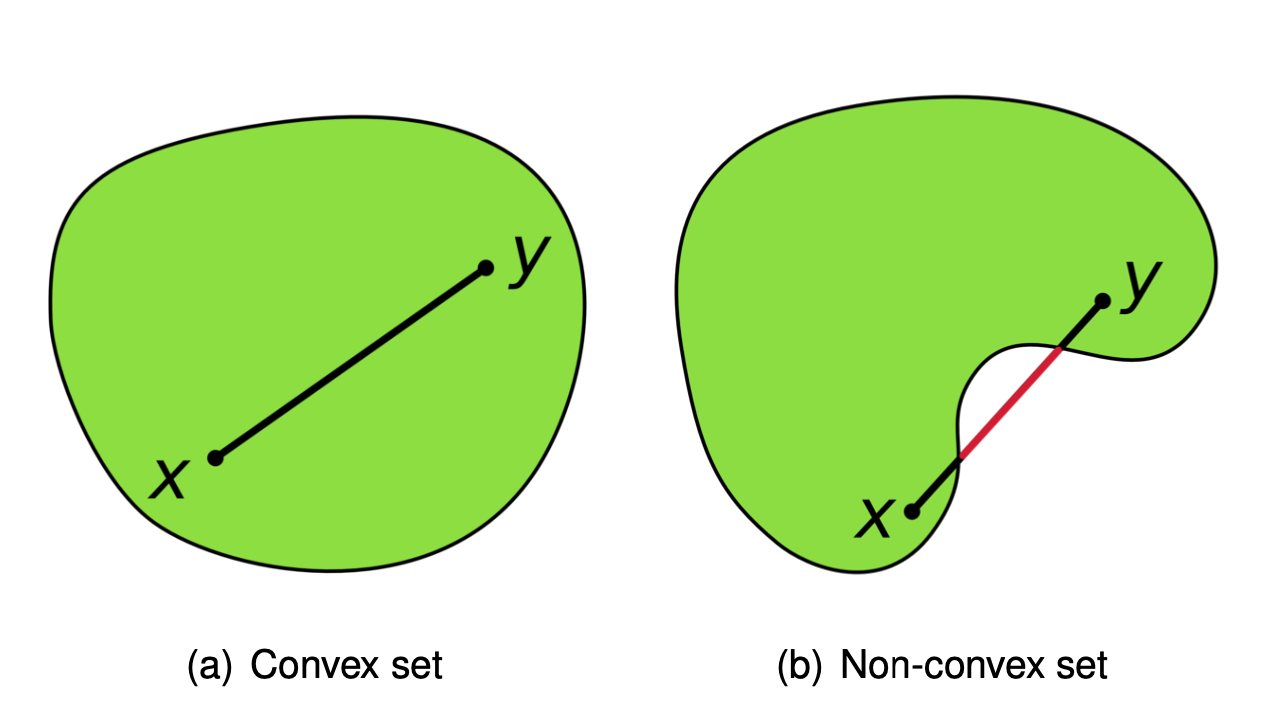
\includegraphics[scale=0.3]{Convex_set.png}
    \caption{}
    \label{}
\end{figure}\end{center}

\begin{claim}
Suppose $f$ is a convex function over $\mathbb{R}^n$ and define the set $$C=\{x\in \mathbb{R}^n| f(x)\leq a\}, a\in \mathbb{R}$$ then $C$ is a convex set.
\end{claim}

\begin{claim}
If $f_1,f_2,...,f_k$ are convex functions over convex set $\&$,
\begin{enumerate}
    \item $f_{sum}(x)=\sum_{i=1}^kf_i(x)$ is convex over $\&$
    \item $f_{max}(x)=\max_{i=1,...,k}f_i(x)$ is convex over $\&$
\end{enumerate}
\end{claim}
\begin{proof}
\quad\\
(2)
\begin{equation}
    \begin{aligned}
        f_{max}(\alpha x+(1-\alpha)y)&=\max_{i=1,...,k}f_i(\alpha x+(1-\alpha)y)\\
    &\leq \max_{i=1,...,k}[\alpha f_i(x)+(1-\alpha)f_i(y)]\\
    &\leq \max_{i=1,...,k}\alpha f_i(x)+\max_{i=1,...,k}(1-\alpha)f_i(y)\\
    &=\alpha f_{max}(x)+(1-\alpha)f_{max}(y)
    \end{aligned}
    \nonumber
\end{equation}
\end{proof}












\subsection{Optimal Conditions}
\begin{proposition}
    Let $f: X \longmapsto \mathbb{R}$ be a convex function over the convex set $X$.

    (a) A local-min of $f$ over $X$ is also a global-min over $X$. If $f$ is strictly convex,then min is unique.

    (b) If $X$ is open (e.g. $\mathbb{R}^{n}$ ), then $\nabla f\left(x^{*}\right)=0$ is a necessary and sufficient condition for $x^{*}$ to be a global minimum.
\end{proposition}
\begin{proof}
\quad\\
Proof based on a property: If $f$ is differentiable over $C$, then $f$ is convex iff
$$
f(z) \geq f(x)+(z-x)^{\prime} \nabla f(x), \quad \forall x, z \in C .
$$
\end{proof}














\begin{corollary}
    Let $f: X \longmapsto \mathbb{R}$ be a concave function over the convex set $X$.

    (a) A local-max of $f$ over $X$ is also a global-max over $X$.

    (b) If $X$ is open (e.g. $\mathbb{R}^{n}$ ), then $\nabla f\left(x^{*}\right)=0$ is a necessary and sufficient condition for $x^{*}$ to be a global maximum.
\end{corollary}


\subsection{$\mu-$strongly convexity}
\textbf{Definition}: We say $f: C \rightarrow \mathbb{R}$ is a $\mu$-strongly convex function in a convex set $C$ if $f$ is differentiable and
$$
\langle\nabla f(w)-\nabla f(v), w-v\rangle \geq \mu\|w-v\|^{2}, \quad \forall w, v \in C .
$$
If $f$ is twice differentiable, then $f$ is $\mu$-strongly convex iff
$$
\nabla^{2} f(x) \succeq \mu I, \quad \forall x \in C .
$$
Namely, all eigenvalues of the Hessian at any point is at least $\mu$.

if $f(w)$ is convex, then $f(w)+\frac{\mu}{2}\|w\|^{2}$ is $\mu$-strongly convex.

- In machine learning, easy to change a convex function to a strongly convex function: just add a regularizer

\subsection{Unconstrained Quadratic Optimization}
$$\begin{array}{ll}\text { minimize } & f(\mathbf{w})=\frac{1}{2} \mathbf{w}^{T} \mathbf{Q} \mathbf{w}-\mathbf{b}^{T} \mathbf{w} \\ \text { subject to } & \mathbf{w} \in \mathbb{R}^{d}\end{array}$$
where $\mathbf{Q}$ is a symmetric $d \times d$ matrix. (what if non-symmetric?)
$$\nabla f(\mathbf{w})=\mathbf{Q}\mathbf{w}-\mathbf{b},\ \nabla^2 f(\mathbf{w})=\mathbf{Q}$$
\begin{enumerate}[(i)]
    \item $\mathbf{Q}\succeq 0 \Leftrightarrow	f$ is convex.
    \item $\mathbf{Q}\succ 0 \Leftrightarrow	f$ is strictly convex.
    \item $\mathbf{Q}\preceq 0 \Leftrightarrow	f$ is concave.
    \item $\mathbf{Q}\prec 0 \Leftrightarrow	f$ is strictly concave.
\end{enumerate}









- Necessary condition for (local) optimality
$$
\mathbf{Q} \mathbf{w}=\mathbf{b}, \quad \mathbf{Q} \succeq 0
$$

Case 1: $\mathbf{Q w}=\mathbf{b}$ has no solution, i.e. $\mathbf{b} \notin R(\mathbf{Q})$. No stationary point, no lower bound ($f$ can achieve $-\infty$).

Case 2: $\mathbf{Q}$ is not PSD ( $f$ is non-convex)
No local-min, no lower bound ($f$ can achieve $-\infty$).

Case 3: $\mathbf{Q} \succeq 0$ (PSD) and $\mathbf{b} \in R(\mathbf{Q})$. Convex, has global-min, 
any stationary point is a global optimal solution.

\begin{example}
    Toy Problem 1: $\min _{x, y \in \mathbb{R}} f(x, y) \triangleq x^{2}+y^{2}+\alpha x y$.
\end{example}
\begin{enumerate}
    \item Step 1: First order condition: $2 x^{*}+\alpha y^{*}=0,2 y^{*}+\alpha x^{*}=0$.
    
    - We get $4 x^{*}=-2 \alpha y^{*}=\alpha^{2} x^{*}$. So $\left(4-\alpha^{2}\right) x^{*}=0$.
    
    - Case 1: $\alpha^{2}=4$. If $x^{*}=-\alpha y^{*} / 2$, then $\left(x^{*}, y^{*}\right)$ is a stationary point.
    
    - Case 2: $\alpha^{2} \neq 4$. Then $x^{*}=0 ; y^{*}=-\alpha x^{*} / 2=0$. So $(0,0)$ is stat-pt.
    \item Step 2: Check convexity. Hessian $\nabla^{2} f(x, y)=\left(\begin{array}{ll}2 & \alpha \\ \alpha & 2\end{array}\right)$.
    
    Eigenvalues $\lambda_{1}, \lambda_{2}$ satisfy $\left(\lambda_{i}-2\right)^{2}=\alpha^{2}, i=1,2$.
    Thus $\lambda_{1,2}=2 \pm|\alpha|$.

    - If $|\alpha| \leq 2$, then $\lambda_{i} \geq 0, \forall i$. Thus $f$ is convex. Any stat-pt is global-min.

    - If $|\alpha|>2$, at least one $\lambda_{i}<0$, thus $f$ is not convex.
    \item Step 3 (can be skipped now): For non-convex case $(|\alpha|>2)$, prove no lower bound.
    
    $f(x, y)=(x+\alpha y / 2)+\left(1-\alpha^{2} / 4\right) y^{2}$. Pick $y=M, x=-\alpha M / 2$, then
    $f(x, y)=\left(1-\alpha^{2} / 4\right) M^{2} \rightarrow-\infty$ as $M \rightarrow \infty$.
\end{enumerate}

Summary:

If $|\alpha|>2$, no global-min, $(0,0)$ is stat-pt;

if $|\alpha|=2$, any $(-0.5 \alpha t, t), t \in \mathbb{R}$ is a stat-pt and global-min;

if $|\alpha|<2,(0,0)$ is the unique stat-pt and global-min.

\begin{example}
Linear Regression
\end{example}
$\text{minimize } f(\mathbf{w})=\frac{1}{2}\left\|\mathbf{X}^{T} \mathbf{w}-\mathbf{y}\right\|^{2}$ subject to $ \mathbf{w} \in \mathbb{R}^{d}$

$n$ data points, $d$ features

- $\mathbf{X}$ may be wide (under-determined), tall (over-determined), or rank-deficient

- Note that comparing with the previous case, $\mathbf{Q}=\mathbf{X X}^{T} \in \mathbb{R}^{d \times d}$, $\mathbf{b}=\mathbf{X} \mathbf{y} \in \mathbb{R}^{d \times 1}$

- $\mathbf{Q} \succeq 0$; Case 2 never happens!

- First order condition $\mathbf{X X}^{\top} \mathbf{w}^{*}=\mathbf{X} \mathbf{y}$.

\quad - It always has a solution; Case 1 never happens!

\textbf{Claim}: Linear regression problem is always convex; it has global-min.

First order condition
$$
\mathbf{X X}^{\top} \mathbf{w}^{*}=\mathbf{X} \mathbf{y}
$$
which always has a solution.

If $X X^{\top} \in \mathbb{R}^{d \times d}$ is invertible (only happen when $n \geq d$ ), then there is a unique stationary point $x=\left(A^{\top} A\right)^{-1} A^{\top} b$. It is also a global minimum.

If $X X^{\top} \in \mathbb{R}^{d \times d}$ is not invertible, then there can be infinitely many stationary points, which are the solutions to the linear equation.
All of them are global minima, giving the same function value.



\section{MATH 484}
A base point $x$, we consider an arbitrary direction $u$. $\{x+tu| t\in \mathbb{R}\}$

We define \underline{the restriction of $f$ to the line through $x$ in the direction of $u$} to be the function:
$$\phi_u (t)=f(x+tu)$$
\begin{lemma}
$x^*$ is a global minimizer of $f$ iff for all $u$, $t=0$ is the global minimizer of $\phi_u (t)$
\end{lemma}
\begin{proof}
\quad\\
($\Rightarrow$) $\phi_u (0)=f(x^*)\leq f(x^*+tu)=\phi_u (t)$\\
($\Leftarrow$) Let $X\in \mathbb{R}^n$, $u=X-x^*$. $\phi_u (0)\leq \phi_u (1) \Rightarrow f(x^*)\leq f(x^*+u)=f(x)$
\end{proof}


\subsubsection{The first-derivative test in $\mathbb{R}^n$: $\phi'_u (t)=\nabla f(x+tu)\cdot u$}
First derivative of $f:\mathbb{R}^n \rightarrow \mathbb{R}$,
Easier: $\phi'_u (t)$?\\
Suppose $f:\mathbb{R}^n \rightarrow \mathbb{R}$ and $\mathsf{g}:\mathbb{R} \rightarrow \mathbb{R}^n$:
$$\frac{\partial f(\mathsf{g}(t))}{\partial t}=\sum_{i=1}^n \frac{\partial f}{\partial x_i}(\mathsf{g}(t))\frac{d}{dt}g_i(t)$$
$$\frac{\partial \phi_u (t)}{\partial t}=\sum_{i=1}^n \frac{\partial f}{\partial x_i}(x+tu)u_i$$

The gradient of $f$: $\nabla f(x)=(\frac{\partial f}{\partial x_1},..., \frac{\partial f}{\partial x_d})^T \Rightarrow \phi'_u (t)=\nabla f(x+tu)\cdot u$

\underline{Fine print}: Chain rule only works when all $\frac{\partial f}{\partial x_k}$ exists and are continuous.\\

\begin{example}
$f(x,y)=x^2+3xy-1,\ x^*=(0,0),\ u=(3,2)$\\
$\phi_u(t)=f(x^*+tu)=f(3t,2t)=27t^2-1$\\
$\phi_u'(t)=54t$\\
$\nabla f(x,y)=(2x+3y, 3x)$\\
$\phi'_u (t)=\nabla f(x+tu)\cdot u= 54t$
\end{example}

\subsubsection{Theorem 4: $\nabla f$ is continuous, $x^*$ is a global minimizer of $f$ $\Rightarrow \nabla f(x^*)=0$}
\begin{theorem}[Theorem 2.1]
    Given a function $f:\mathbb{R}^n \rightarrow \mathbb{R}$, if $\nabla f$ is continuous and $x^*$ is a global minimizer of
    $f$, then $\nabla f(x^*)=0$. (When $\nabla f(x^*)=0$, we call $x^*$ a \underline{critical point} of $f$.)
\end{theorem}
$x^*$ is a global minimizer $\Rightarrow$ $x^*$ is a critical point, inverse may not true.

\subsubsection{The second-derivative test in $\mathbb{R}^n$}
$$\phi'_u (t)=\sum_{i=1}^n \frac{\partial f}{\partial x_i}(x+tu)u_i$$
$$\phi^{''}_u (t)=\sum_{i=1}^n \sum_{j=1}^n u_iu_j\frac{\partial^2 f}{\partial x_i\partial x_j}(x+tu)$$
\subsubsection{Hessian matrix}
Define Hessian matrix of $f$ and write $Hf$. That is,

$$\phi^{''}_u (t)=u^T Hf(x+tu) u$$
\underline{Fine print}: Chain rule only works when all $\frac{\partial^2 f}{\partial x_i\partial x_j}$ exists and are continuous. ($\Rightarrow$ $Hf$ is continuous)\\

\subsubsection{Theorem 5: $Hf$ is continuous, $\nabla f(x^*)=0$, $u^T Hf(x^*) u\geq 0,\forall u$ $\Rightarrow$ $x^*$ is a global minimizer of $f$}
\begin{theorem}
    Given a function $f:\mathbb{R}^n \rightarrow \mathbb{R}$, if $Hf$ is continuous and $x^*$ is a critical point of
    $f$. If for any $u$, that $u^T Hf(x^*) u\geq 0$. Then $x^*$ is a global minimizer of $f$.
\end{theorem}
proved by Taylor
\begin{theorem}[Taylor]
    Given a function $f:\mathbb{R}^n \rightarrow \mathbb{R}$, if $Hf$ is continuous and $x^*$ is a critical point of $f$, then
    $$f(x)=f(x^*)=\nabla f(x^*)(x-x^*)+\frac{1}{2}(x-x^*)^T Hf(z) (x-x^*)$$
for some $z$ on the line between $x$ and $x^*$
\end{theorem}





\subsection{Minimizing over other sets}
What if the domain of $f$: $D\subset \mathbb{R}^n$\\
(1): want $x^*$ to be in the interior of $D$, not on the boundary (want to be able to "look" from $x^*$ in any direction.)\\
(2): want $x^*$ to "see" all other points in $D$ using straight line $u$.\\
Convexity\\
good domain e.g. Ball: $B(x^*,r)=\{x| ||x-x^*||<r \}$

\subsubsection{Theorem 7: $\nabla f$ is continuous, $x^*$(interior of $D$) is a local minimizer of $f$ $\Rightarrow \nabla f(x^*)=0$}
\begin{theorem}[Theorem 4.1, 类似Theorem 2.1]
    Suppose $f: D \rightarrow\mathbb{R}$ has continuous $\nabla f$ and $x^*$ is not on the boundary of $D$. If $x^*$ is a local minimizer of $f$, then $x^*$ is a critical point of $f$: $\nabla f(x^*)=0$
\end{theorem}

\subsubsection{Theorem 8: $Hf$ is continuous, $x^*$(interior of $D$) $\nabla f(x^*)=0$, $\exists r$ s.t. $u^T Hf(x^*) u\geq 0, \forall x\in B(x^*,r),\forall u$ $\Rightarrow$ $x^*$ is a local minimizer of $f$}
\begin{theorem}
    Given a function $f: D \rightarrow\mathbb{R}$ , if $Hf$ is continuous and $x^*$ is a critical point of
    $f$ in the interior of $D$. Suppose $\exists r$ s.t. for any $u$, that $u^T Hf(x^*) u\geq 0$ whenever $x\in B(x^*,r)\subset D$. Then $x^*$ is a local minimizer of $f$.
\end{theorem}




































\end{document}